\begin{figure}[h!]
    \centering
    \caption{Type of living units by (residualized) household income decile}
    \label{fig:ahs_unit_types}

    \begin{subfigure}{.75\textwidth}
        \caption{Share of unit type}
        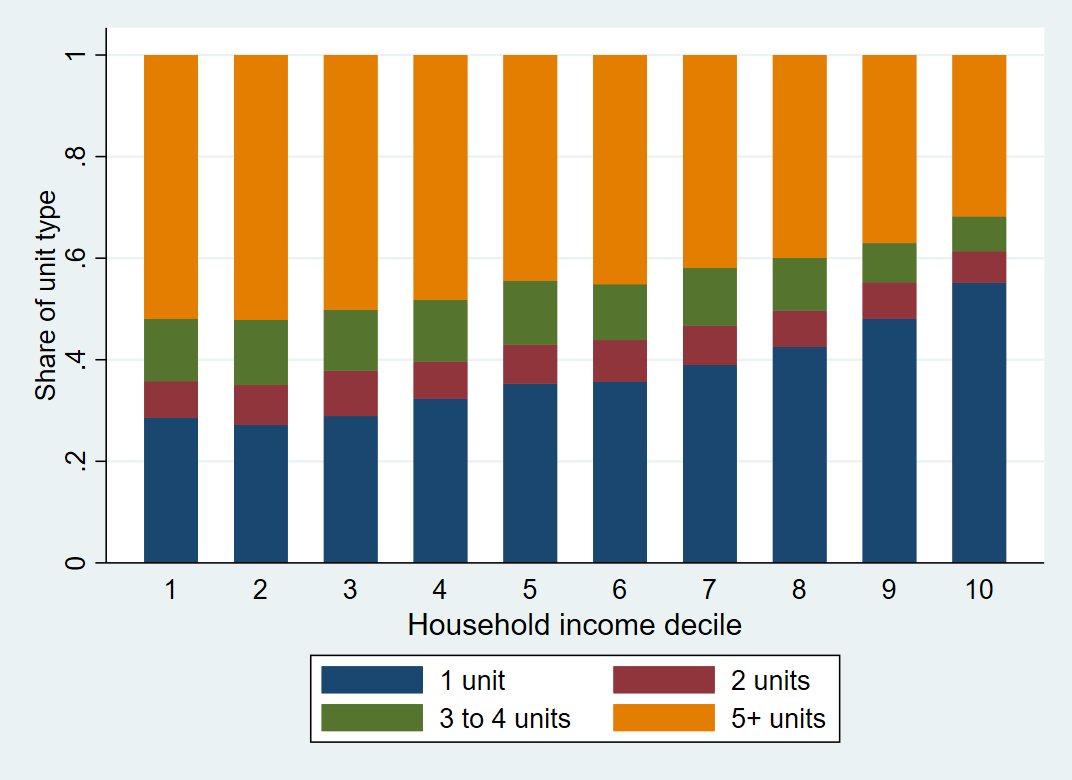
\includegraphics[width = 1\textwidth]
            {ahs/output/sh_unit_types}
    \end{subfigure}\\
    \begin{subfigure}{.75\textwidth}
        \caption{Share of condominiums or cooperative houses}
        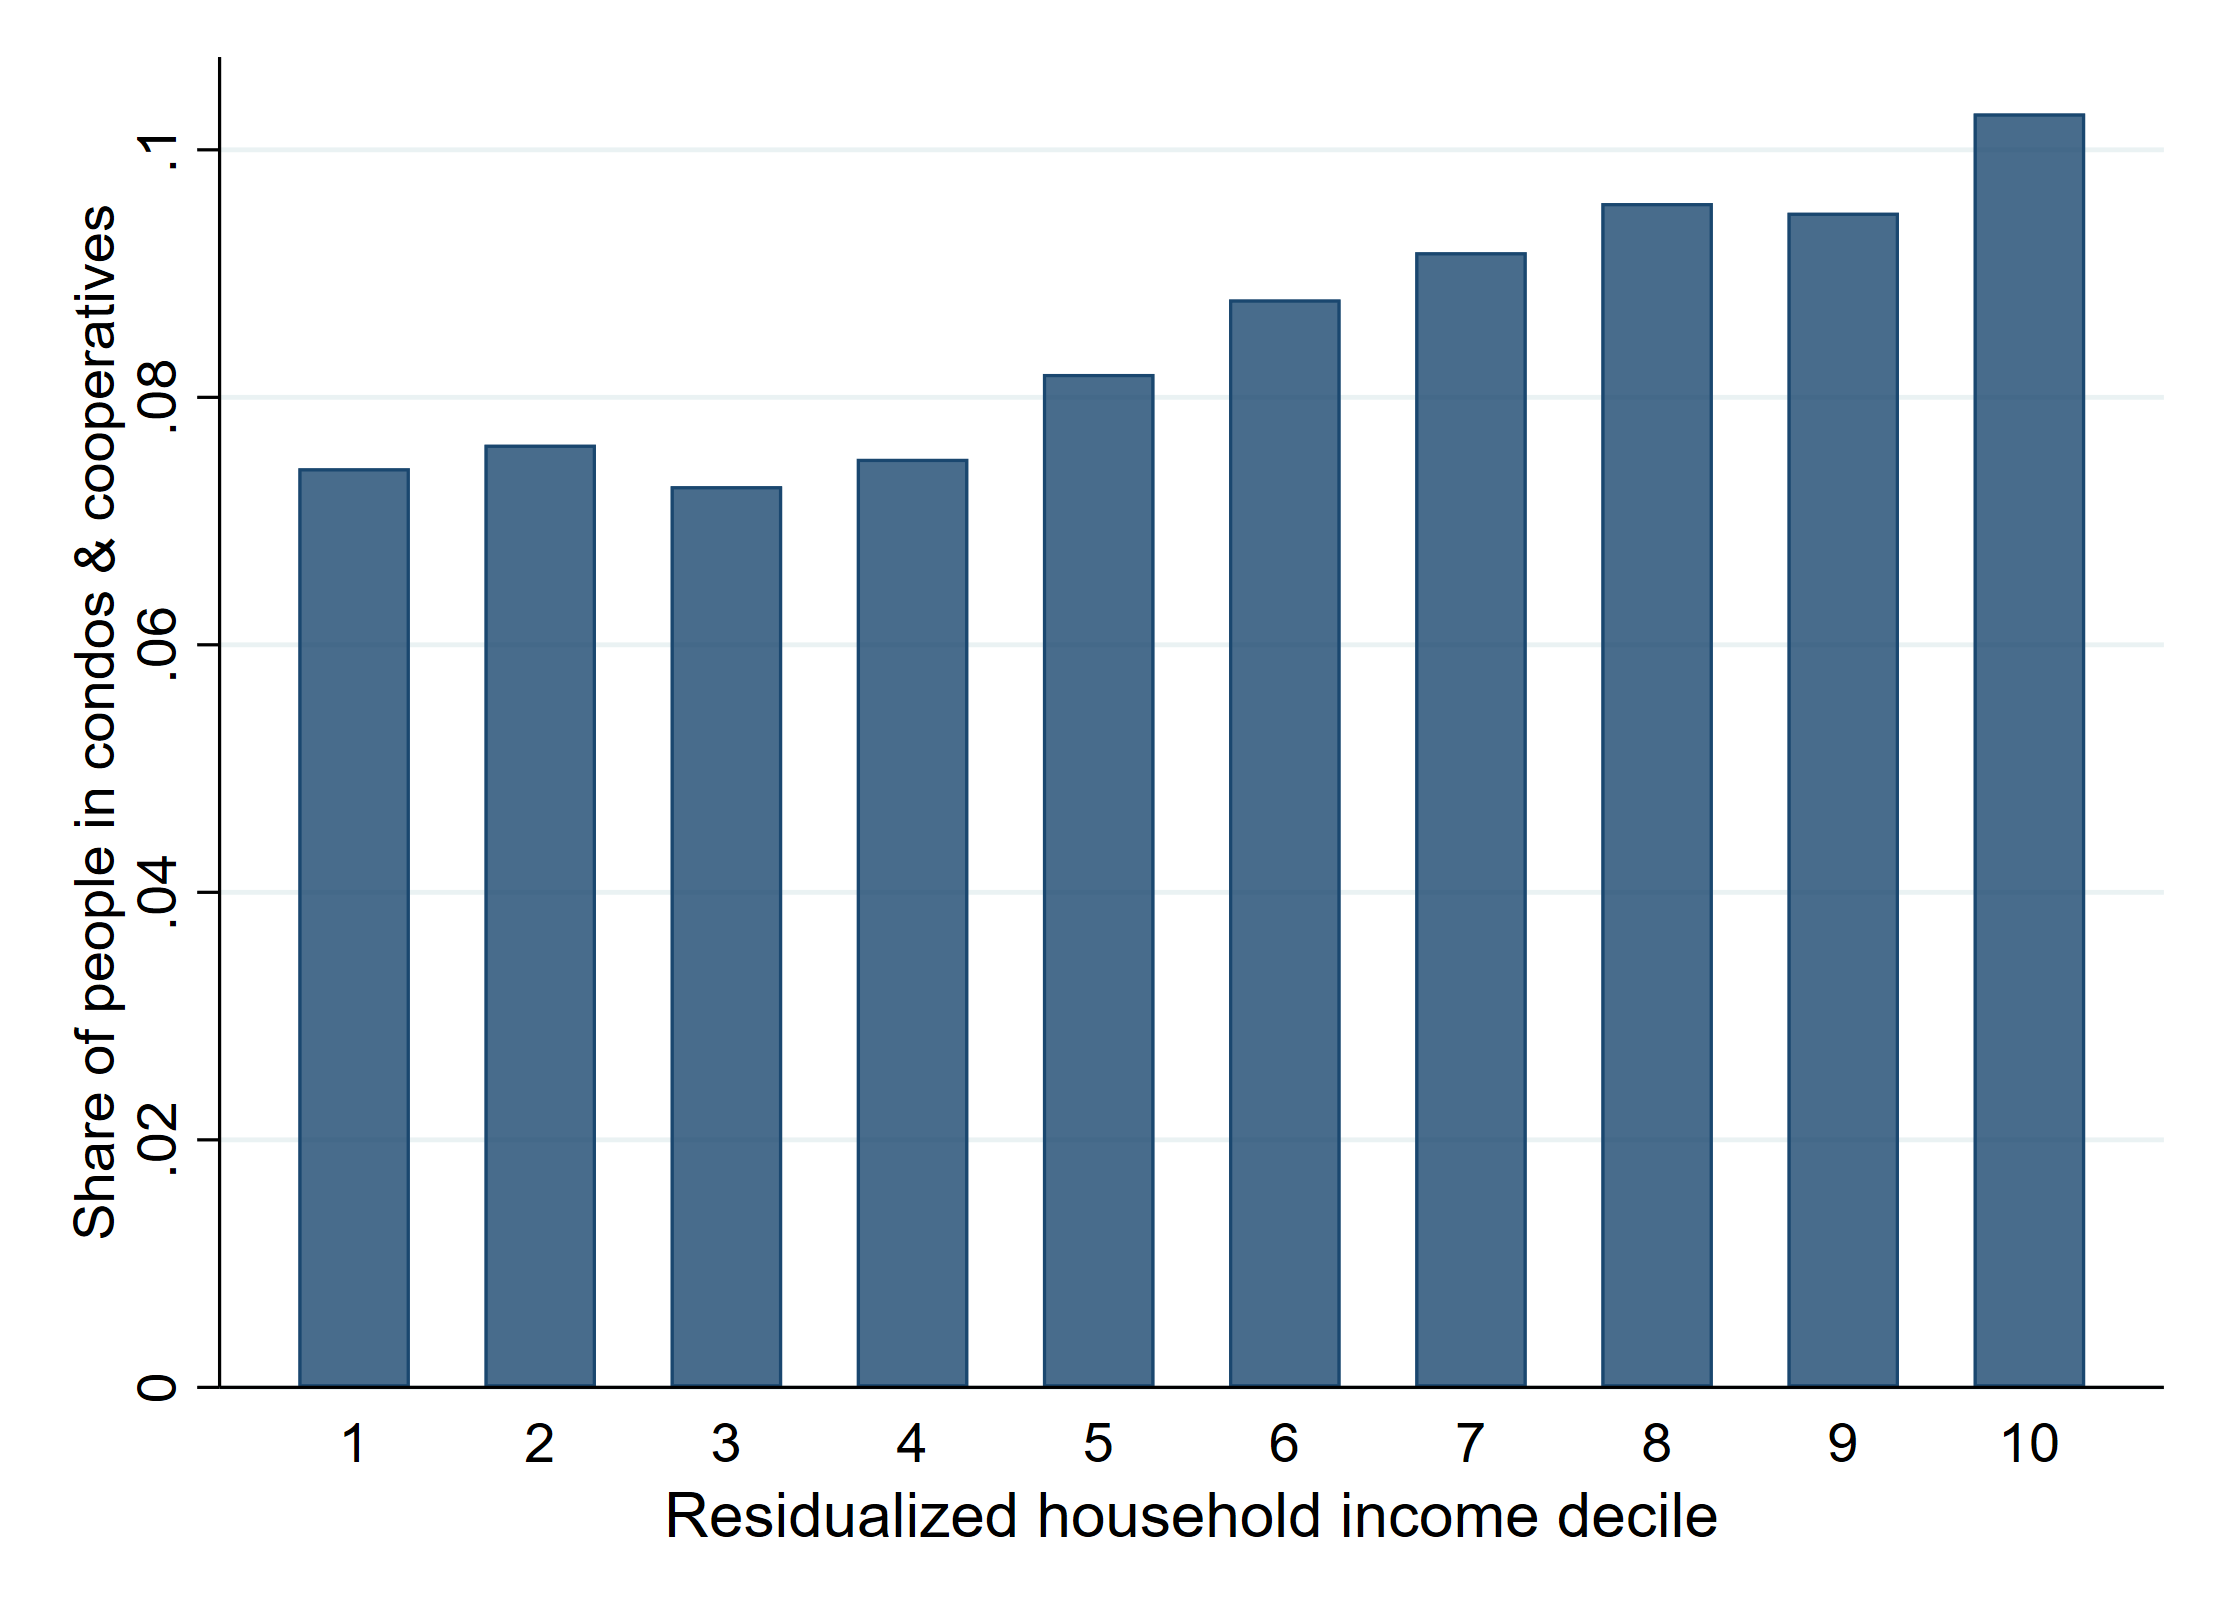
\includegraphics[width = 1\textwidth]
            {ahs/output/sh_condo}
    \end{subfigure}%

    \begin{minipage}{.95\textwidth} \footnotesize
        \vspace{3mm}
        Notes: Data are from the 2011 and 2013 American Housing 
        Survey (AHS), as described in Section \ref{ADD SECTION}. 
        The top figure shows the share of unit types by household
        income, and the bottom figure shows the share of condominiums
        or cooperative houses by household income.
        All of the variables are residualized at the SMSA level.
        We exclude from the calculation non-conventional housing units, 
        such as mobile homes, hotels, rooming houses, etc.
    \end{minipage}
\end{figure}
